%%%%%%%%%%%%%%%%%%%%%%% file template.tex %%%%%%%%%%%%%%%%%%%%%%%%%
%
% This is a general template file for the LaTeX package SVJour3
% for Springer journals.          Springer Heidelberg 2010/09/16
%
% Copy it to a new file with a new name and use it as the basis
% for your article. Delete % signs as needed.
%
% This template includes a few options for different layouts and
% content for various journals. Please consult a previous issue of
% your journal as needed.
%
%%%%%%%%%%%%%%%%%%%%%%%%%%%%%%%%%%%%%%%%%%%%%%%%%%%%%%%%%%%%%%%%%%%
%
% First comes an example EPS file -- just ignore it and
% proceed on the \documentclass line
% your LaTeX will extract the file if required
\begin{filecontents*}{example.eps}
%!PS-Adobe-3.0 EPSF-3.0
%%BoundingBox: 19 19 221 221
%%CreationDate: Mon Sep 29 1997
%%Creator: programmed by hand (JK)
%%EndComments
gsave
newpath
  20 20 moveto
  20 220 lineto
  220 220 lineto
  220 20 lineto
closepath
2 setlinewidth
gsave
  .4 setgray fill
grestore
stroke
grestore
\end{filecontents*}
%
\RequirePackage{fix-cm}
%
%\documentclass{svjour3}                     % onecolumn (standard format)
%\documentclass[smallcondensed]{svjour3}     % onecolumn (ditto)
% \documentclass[smallextended]{svjour3}       % onecolumn (second format)
\documentclass[twocolumn]{svjour3}          % twocolumn
%
\smartqed  % flush right qed marks, e.g. at end of proof
%
\usepackage{graphicx}
%
\usepackage{mathptmx}      % use Times fonts if available on your TeX system
\usepackage{subcaption}
\captionsetup{compatibility=false}
%
% insert here the call for the packages your document requires
%\usepackage{latexsym}
% etc.
%
% please place your own definitions here and don't use \def but
% \newcommand{}{}
%
% Insert the name of "your journal" with
\journalname{Virtual Reality}
%
\begin{document}

\title{FaceAtlasAR: Atlas of Facial Acupuncture Points in Augmented Reality}
% \subtitle{Do you have a subtitle?\\ If so, write it here}

%\titlerunning{Short form of title}        % if too long for running head

\author{Menghe Zhang \and J\"urgen P. Schulze \and Dong Zhang}

%\authorrunning{Short form of author list} % if too long for running head

\institute{Menghe Zhang
\at Department of Computer Science, University of California, San Diego, CA, USA,\\
\email{mez071@eng.ucsd.edu}
\and
J\"urgen P. Schulze
\at Department of Computer Science, University of California, San Diego, CA, USA,\\
\email{jschulze@ucsd.edu}
\and
Dong Zhang
\at Qilu University of Technology, Shandong, China,\\
\email{jnzd156@163.com}
}

\date{Received: date / Accepted: date}
% The correct dates will be entered by the editor

\maketitle

\begin{abstract}
Acupuncture is a technique in which practitioners stimulate specific points on the body. Those points, called acupuncture points (or acupoints), anatomically define areas on the skin relative to specific landmarks on the body. However, mapping the acupoints to individuals could be challenging for inexperienced acupuncturists. In this project, we proposed a system to localize and visualize facial acupoints for individuals in an augmented reality (AR) context. This system combines a face alignment model and a hair segmentation model to provide dense reference points for acupoints localization in real-time (60FPS). The localization process takes the proportional bone (B-cun or skeletal) measurement method, which is commonly operated by specialists; however, in the real practice, operators sometimes find it inaccurate due to the skill-related error. With this system, users, even without any skills, can locate the facial acupoints as a part of the self-training or self-treatment process.
\keywords{Augmented reality \and Acupuncture point \and Face alignment \and Hair segmentation}
% \PACS{PACS code1 \and PACS code2 \and more}
% \subclass{MSC code1 \and MSC code2 \and more}
% \CRclass{10010392 \and }
\end{abstract}

\section{Introduction}
\label{intro}
Acupuncture\cite{li2015acupoint} is a form of alternative medicine and a key component of traditional Chinese medicine (TCM). Based on the symptoms, acupuncturists stimulate specific anatomic sites commonly by needling, massaging, or heat therapy. Scientific studies have proved that acupuncture may help ease types of pain that are often chronic such as low-back pain, neck pain, and osteoarthritis/knee pain. The acupoints on the face can help with a variety of conditions both on and off the face, such as jaw tension, headaches, anxiety, and stomach conditions.
\\
However, acupuncture practice relies on experienced acupuncturists to locate the acupoints from body acupuncture maps. Individuals, who want to help themselves relieve symptoms with acupoints stimulation, usually find it confusing to localize the targets by natural language description or pictures of a standard model.
\\
With the help of augmented reality, we designed a system to display facial acupoints on the top of the user’s face to accurately view and localize facial acupuncture points. Specifically, we employ a deep learning model to annotate 3D landmarks and on a user’s face together with hair segmentation in real-time to gather reference points for acupuncture points localization. We then align the reference point with acupuncture points defined by proportional bone measurement method. The whole process is implemented via MediaPipe, a framework for building cross-platform machine learning solutions. Our system works perfectly on phones with a front camera, without any extra hardware, users could pinpoint and interact with the target acupoints. There are three benefits to this application:
\begin{itemize}
  \item It takes a conventional localization method while originally defines a scheme to transform the natural language descriptions to mathematical logic expressions.
  \item It adopts MediaPipe framework to run across platforms in real-time.
  \item It adapts to different head poses to be robust for users to locate acupoints in different regions.
\end{itemize}
With FaceAtlasAR, people who have little or no experience in localizing facial acupuncture points can use. Potential use scenarios for our applications are varied, for example, acupuncture education, communication, and self-healing.

\section{Related Work}
\label{sec:related-work}
\subsection{Acupuncture point localization}
\label{sec:related-acu-localize}
Existing works of acupuncture training applications on AR devices are limited. In 2015, H. Jiang et al.\cite{li2015acupoint} proposed the first acupuncture training application, Acu Glass, on a head-mount display device(HMD) based on Google Glass. They generated the frontal face acupoints based on the height and the width of the input face, plus the distance between the eyes. However, their face landmarks for reference are too limited to adapt to different people and different poses of the face. Other acupoints localization methods like Chen et al.\cite{chen2017localization}\cite{lan2018toward} fit a 3D Morphable Face Model(3DMM)\cite{huber2016multiresolution} to a 2D image, and combine facial landmarks and image deformation to estimate acupoints. 3DMM is a powerful tool to build polygonal mesh though, the range of possible predictions is limited by the linear manifold spanned by the PCA basis, which is in turn determined by the diversity of the set of faces captured for the model\cite{kartynnik2019real}. Therefore, manual annotation on a standard 3D model may not correctly fit all kinds of people. Moreover, acupoints are officially defined relative to landmarks, while the deformation process does not guarantee the relativeness.\\
As for the localization methods in practice, Godson and Wardle\cite{godson2019accuracy} screened 771 studies and summarized the methods as Directional(F-cun) method, Proportional method, palpation for tenderness, electronic point detectors, and anatomical locations. Usually, more accurate approaches are the next steps of less accurate ones and require extra hardware. For example, one can roughly locate a target by the directional method and then use electronic point detectors to measure the electrical resistance of the skin. There are researches related to this topic and acupoint probing devices available in the market.

\subsection{Face alignment}
\label{sec:related-face-align}
Face alignment is a computer vision technology for identifying the geometric structure of human faces in digital images. Bulat and Tzimiropoulos\cite{bulat2017far} reviewed 2D and 3D face alignment and landmark localization. Existing 2D and 3D datasets annotate a limited set of landmarks. For example, 300-W\cite{sagonas2013semi}, the most widely-used in-the-wild dataset for 2D alignment, containing LFPW\cite{belhumeur2013localizing}, HELEN\cite{le2012interactive}, AFW\cite{zhu2012face}, and iBUG\cite{sagonas2013semi}, annotates only 68 landmarks per face. These landmarks either have distinct semantics of their own or participate in meaningful facial contours. Works based on them are not suitable for our cases. We finally adopted the work of Kartynnik et al.\cite{kartynnik2019real}, which estimates 3D mesh with 468 vertices in real-time. The vertices are selected manually according to expressive AR effects, thus well suitable for our requirements.

\section{System Overview}
Our facial localization solution utilizes the MediaPipe machine learning pipeline consisting of an off-line stage and an on-line stage(Fig.\ref{fig:structure}).
\begin{figure}
\centering
  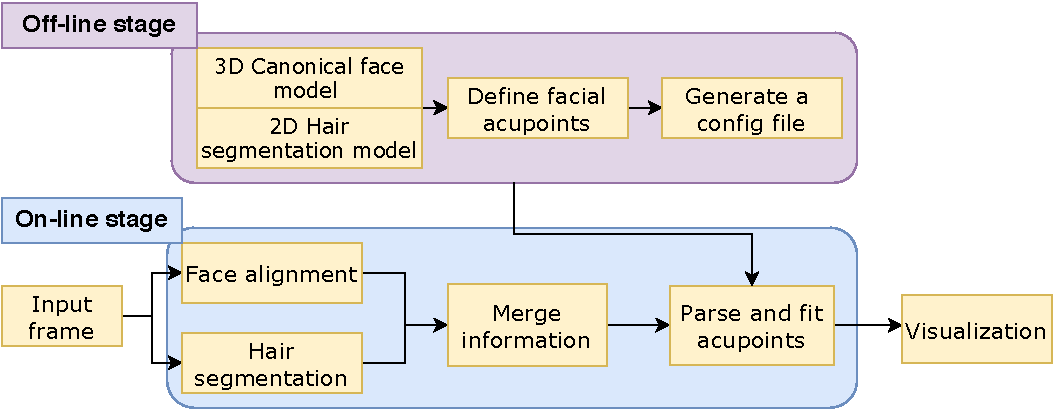
\includegraphics[width=0.9\columnwidth]{figures/structure.pdf}
  \caption{Workflow of the proposed system}~\label{fig:structure}
\end{figure}

During the off-line stage:
\begin{itemize}
\item \textbf{Model selection:} BBased on the definition of the referenced points on a face, we choose to blend a pre-trained face alignment model and a pre-trained hair segmentation model. This is because a single model cannot cover the whole set of target regions, while different parts of the regions are in the different reference systems.
\item \textbf{Acupoints localization:} We firstly localize facial anatomical landmarks, which are designated by the National Standard of the People’s Republic of China. We then use the proportional bone (B-cun or skeletal) measurement method to locate all acupoints on the face.
\item \textbf{Data file generation:} The file contains all the information needed for each acupoint/reference point, including name, region, relative location towards a landmark or a reference point. The file is readable for non-technical users, for example, acupuncturists, to correct less accurate acupoint descriptions by natural language.
\end{itemize}

Then at the on-line stage, the system gets face landmarks together with hair segmentation and merges those results into acupoints generator. The generator gives out the requested acupoints on this frame based on the prior knowledge and then draw on the input face.\\
We fit the whole process into MediaPipe’s perception pipeline as a graph of modular components. Each component, called Calculator, solves an individual task like model inference, data transformation, or annotation. We will talk about the implementation details in the next section. We show the graph for our FaceAtlasAR in Figure  \ref{fig:graph_main}.\\
\begin{figure}
\centering
  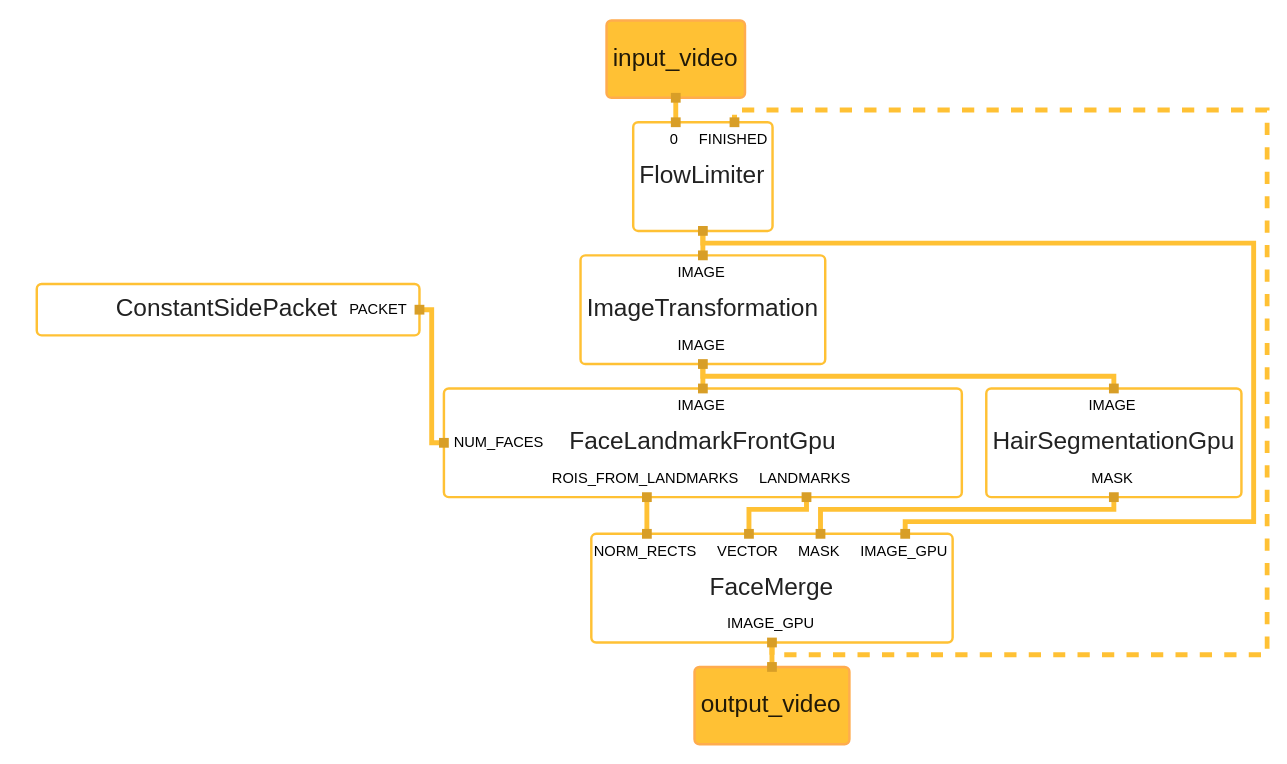
\includegraphics[width=\columnwidth]{figures/graph_main.png}
  \caption{The graph of FaceAtlasAR}~\label{fig:graph_main}
\end{figure}
The graph consists of two subgraphs: one for face alignment (FaceLandmarkFrontGpu) and the other for hair segmentation (HairSegmentationGpu). From the graph, we see the FlowLimiter guards the whole pipeline process. By connecting the output of the final image to the FlowLimiter with a backward edge, the FlowLimiter keeps track of how many timestamps are currently being processed. The system will down-sample and transform the original image before fusing the input to machine learning models but will draw the results onto the original frames. The next section will show the implementation of each module in detail.

\section{Implementation}
\label{sec:implementation}

\subsection{Face alignment}
\label{sec:implement-face-alignment}
We adopted a pre-trained TFLite model\cite{kartynnik2019real} to infer an approximate 3D mesh representation of a human face.\\
This process comprises of majorly three steps:
\begin{itemize}
    \item \textbf{Face detection}: The whole frame is first processed by a lightweight face detector to get the face bounding box and several landmarks, thus, to get the rotation matrix of the face. This step only runs until the system finds a face to track or when the system loses tracking.
    \item \textbf{Image transformation}: The image is then cropped by the bounding box and resized to fit into the next step. After this step, the target region is centered and aligned.
    \item \textbf{Face landmarks generation}: The pre-trained model produces a vector of 3D landmark coordinates, which subsequently gets mapped back into the original image coordinate system.
\end{itemize}
Then from a canonical face mesh model, we extract those vertices with semantic meaning as the reference points(Fig.\ref{fig:face_mesh}).
\begin{figure}
  \centering
    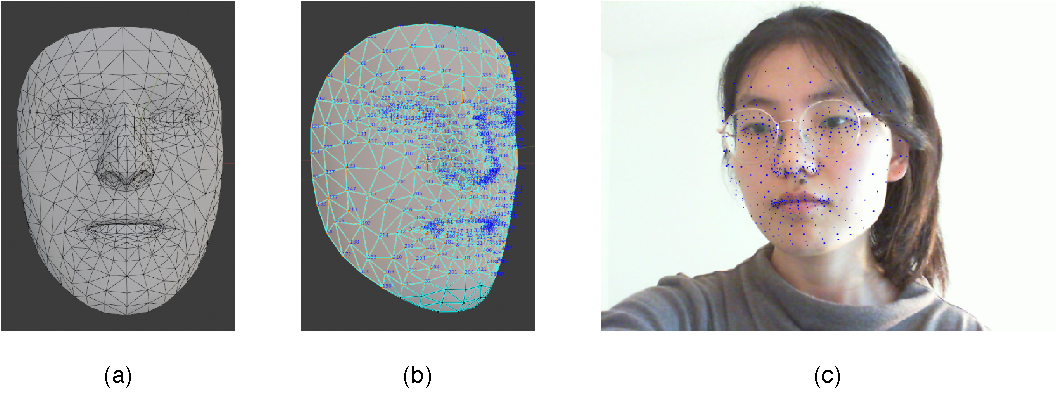
\includegraphics[width=0.9\columnwidth]{figures/facemesh.pdf}
    \caption{The generated mesh topology(a), its vertices with index(b), and viewed in AR(c)}~\label{fig:face_mesh}
  \end{figure}

\subsection{Hair segmentation}
\label{sec:implement-hair-segmentation}
Since the center of the frontal hairline is a critical facial anatomical landmark according to the national standard, we adopted a pre-trained model\cite{tkachenka2019real} to get the hair segmentation mask. Similar to the face alignment process, the previously generated mask can be fed back to help accelerate the process. Specifically, the mask from the previous round of inference will be embedded as the alpha channel of the current input image(Fig.\ref{fig:hair_seg}).
\begin{figure}
  \centering
    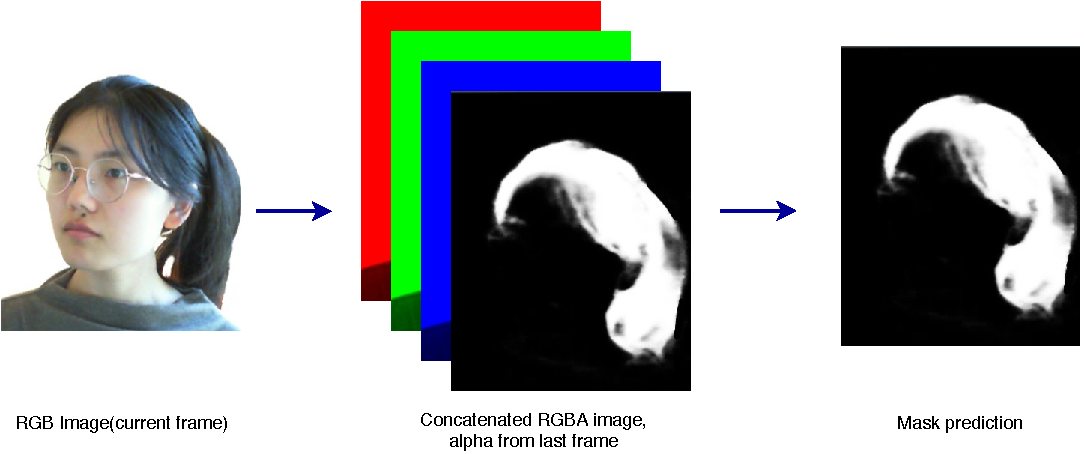
\includegraphics[width=0.9\columnwidth]{figures/hair.pdf}
    \caption{Hair segmentation module}~\label{fig:hair_seg}
\end{figure}

\subsection{Facial acupoints definition}
\label{sec:implement-facial-acu-define}
Given the hair mask together with face landmarks, we now could locate facial acupoints based on the B-cun method. This refers to the method of measuring the length and width of each part of the body with the body surface condyles as the main landmark and determining the position of acupoints. Then, a unit “cun” is the length between the set two bone nodes divided into certain equal parts as the basis for setting acupoints. The facial acupoints bank on the unit cun’s definition of the head as shown in Fig.\ref{fig:cun}. 
\begin{figure}
  \centering
  \begin{subfigure}[t]{0.45\columnwidth}
      \centering
      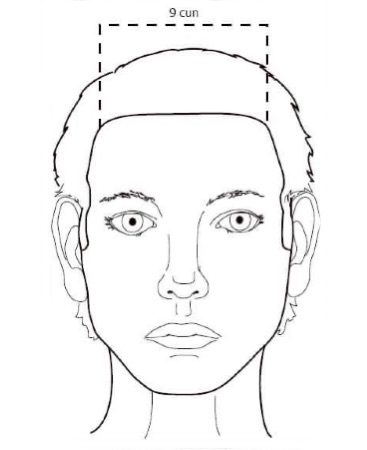
\includegraphics[width=\textwidth]{figures/b-cun-2.jpg}
      \caption{B-cun on the font face}
      \label{fig:cun-front}
  \end{subfigure}%
  ~ 
  \begin{subfigure}[t]{0.45\columnwidth}
      \centering
      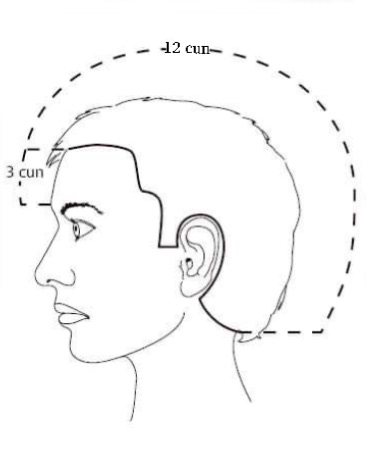
\includegraphics[width=\textwidth]{figures/b-cun.jpg}
      \caption{B-cun on the side face}
      \label{fig:cun-side}
  \end{subfigure}
  \vskip 0.15in
  \caption{B-cun on the head from National Standard of the People's Republic of China, Acupoints\protect\cite{jingxuebiaozhun}. Pictures from\protect\cite{musculoskeletalkey}.}
  \label{fig:cun}
\end{figure}
To start with, we locate three facial anatomical landmarks in consonance with the national standard. In order to differentiate these three points to acupoints, we group them in the channel named RHD:
\begin{itemize}
  \item \textbf{RHD1,Yintang}: The midway between the medial ends of the eyebrows.
  \item \textbf{RHD2,Middle of anterior hairline}: Intersection of anterior hairline and anterior midline.
  \item \textbf{RHD3,Pupils}
\end{itemize}


From Fig.\ref{fig:cun-side}, the distance from Yintang to Middle of anterior hairline, $d_{RHD1->RHD2}$ decides the unit cun as $uc=d_{RHD1->RHD2}/3$. On that occasion, like RHD points definition, we could locate all facial acupoints. Table\ref{tab:acu-info} shows an example of what information we keep for each acupoint. All points’ information finally makes up to a data file.

\begin{table}
\begin{center}
\begin{tabular}{c|c|c|c}
\hline
Channel Name & ID & NameE & Region \\
\hline
ST& 2& Sibai & eye\\
\hline
\hline
FaceMeshX & FaceMeshY & IsSymmetry & Comments \\
\hline
GetX(RHD3)& GetY(ST1)+0.5*U & TRUE & - \\
\hline
\end{tabular}
\end{center}
\caption {Information of an example acupoint Sibai(ST2) in the data file.} 
\label{tab:acu-info} 
\end{table}
There is one more aspect we want to specify, the channel name, which refers to a unique meridian channel. The meridian system is a concept in TCM about a path through which the life-energy is known as "qi" flows. There are 12 standard and 8 extraordinary meridians, while acupoints are the chosen sites on the meridian system. So we group the acupoints on the same meridian channel and connect them by the flow. For example, the previously stated acupoint, Sibai, belongs to the ST(Foot's Yang Supreme Stomach Meridian) channel. Acupoints on the ST channel and their flow are illustrated in the Fig.\ref{fig:st_channel}.
\begin{figure}
\centering
  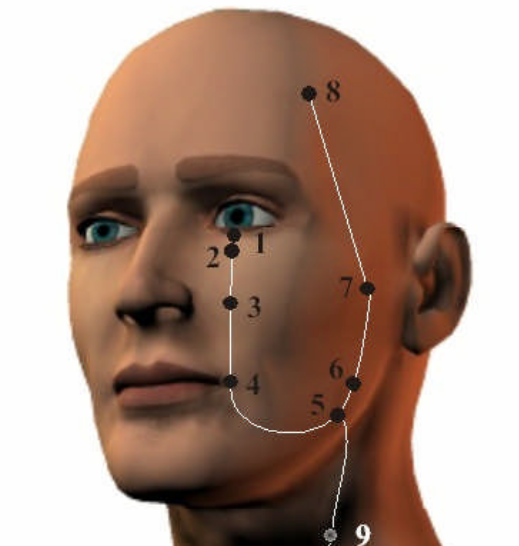
\includegraphics[width=0.8\columnwidth]{figures/st.png}
  \caption{Illustration of ST channel on the head. Picture from \protect\cite{stchannel} }~\label{fig:st_channel}
\end{figure}

\section{Results}
\label{sec:results}
We achieve real-time performance on both desktop and mobile devices by designing the pipeline properly. We show the final application below and compare the performance on different platforms.

\subsection{Android Application}
\label{sec:res-android-app}
Figure \ref{fig:res} presents the screenshots from our FaceAtlasAR android app. Here we show the visualization of acupoints grouped by meridian channels in different poses. Thanks to the robustness of face alignment towards occlusion, users would not find problems pointing or pressing a target acupoint(Fig.\ref{fig:press}).
\begin{figure}
  \centering
    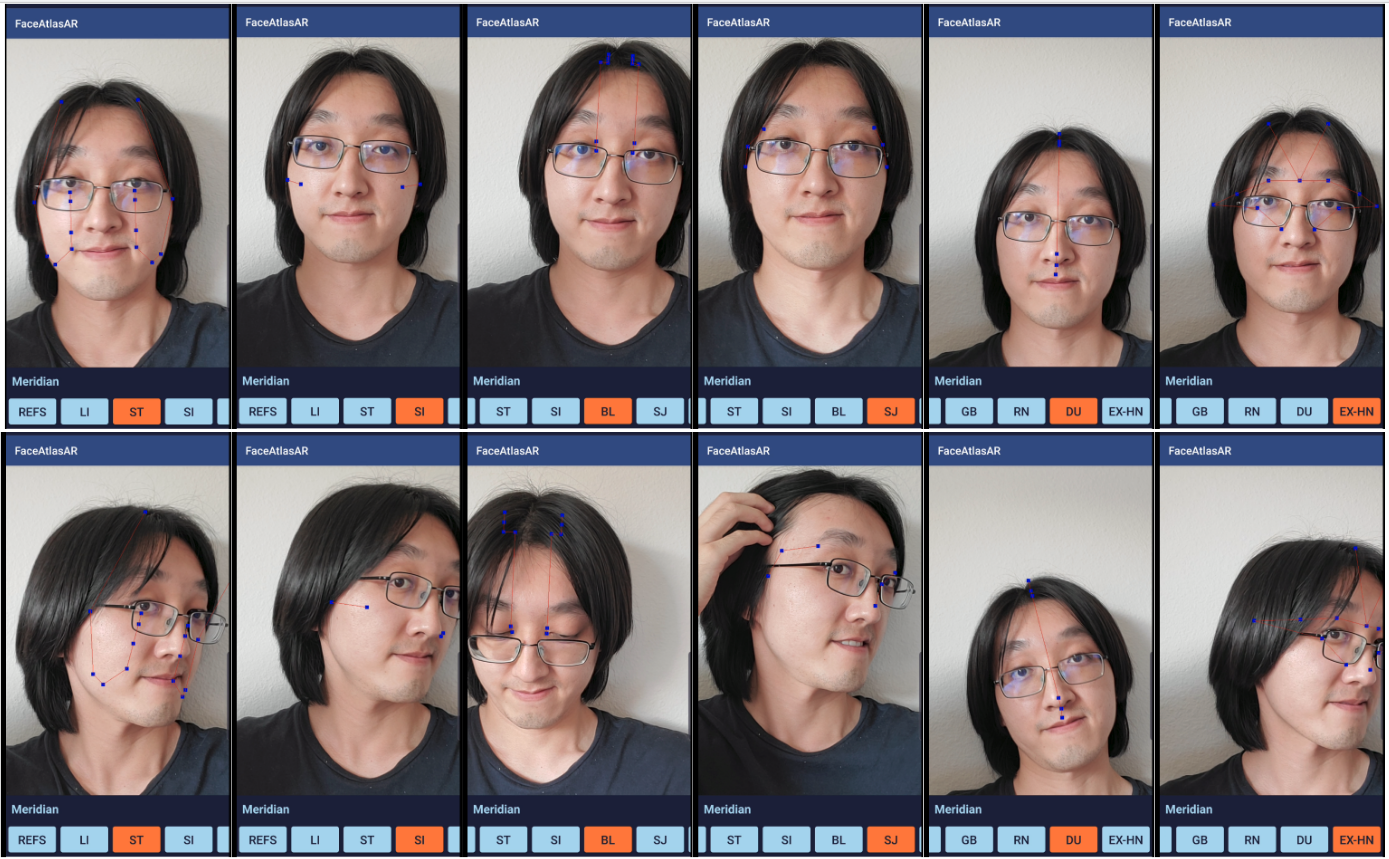
\includegraphics[width=\columnwidth]{figures/res.png}
    \caption{Android application screenshots for displaying acupoints grouped by meridian system in different poses}~\label{fig:res}
  \end{figure}
\begin{figure}
  \centering
    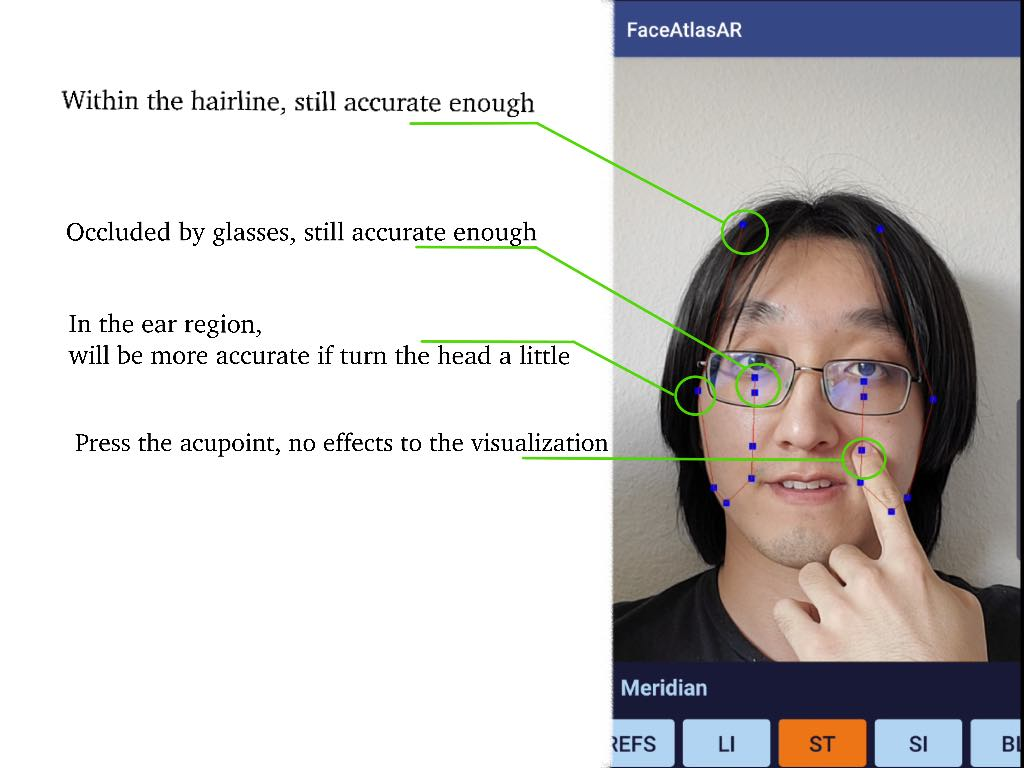
\includegraphics[width=\columnwidth]{figures/press-acu.jpg}
    \caption{User presses an acupoint on ST meridian channel}~\label{fig:press}
  \end{figure}

\subsection{Accuracy}
\label{sec:res-accuracy}
We setup an experiment on Samsung S10(2280$\times$1080) to valid the accuracy of our FaceAtlasAR to localize 4 reference points and 69 acupuncture points on face by comparing the mean pixel errors between ground truth positions and the localization results. Initially, we assign all the target positions into three groups by the localization complexity as shown in the Table \ref{tab:acupoint-cat}.
\begin{table}
\caption{Acupoints categorized by localization times}
\begin{center}
\begin{tabular}{p{0.15\columnwidth}|p{0.15\columnwidth}|p{0.22\columnwidth}|p{0.22\columnwidth}}
\hline
Method & Direct & One-time proportional& Multiple-times proportional\\
\hline
Reference points &3& 1  & 1\\
\hline
Acupoints & 38 & 16 &15 \\
\hline
\end{tabular}
\end{center}
\label{tab:acupoint-cat}
\end{table}

We then investigate the mean pixel errors in 3 groups. For each localization points, we measure the pixel errors in 4 different poses: frontal face ($0^{\circ}$), pitch (X-axis$+10^{\circ}$), roll (Y-axis $+10^{\circ}$), yaw (Z-axis $+10^{\circ}$) to get the mean value. The results are shown in Figure \ref{fig:mean-pixel-err}.
\begin{figure}
  \centering
    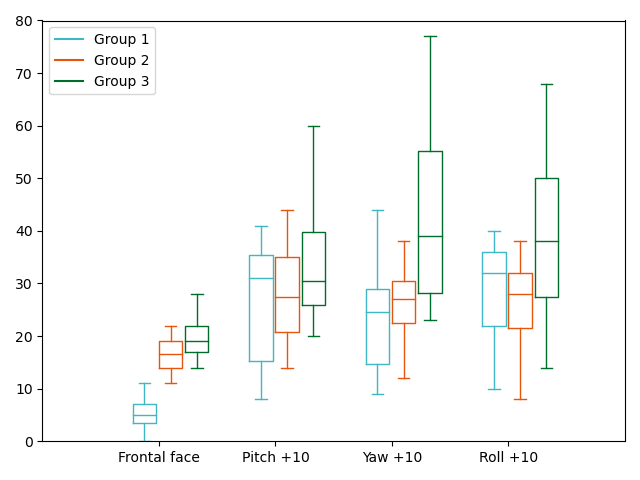
\includegraphics[width=\columnwidth]{figures/mean_pixel_err.png}
    \caption{Mean pixel errors of localization}~\label{fig:mean-pixel-err}
  \end{figure}

From the results we found that some of the localizations are less precise than others. Especially, the system performs worse on group 2 than group 1 and group 3 than group 2. Accordingly, multiple times of proportional calculations that rely on the cun system add inaccuracy to the results. The system tolerates to different angles to some extent. However, a target point will be more well localized when it is point straight to the camera without any angles.

\subsection{Performance}
\label{sec:res-performance}
We evaluate the performance of our pipeline in three major components: face alignment, hair segmentation, and acupoints generation. Since the application runs on multiple platforms, we compare its performance on a desktop with Nvidia GeForce RTX 2070 SUPER and on a Samsung S10. The input images for two TFLite models are both in full size 512$\times$512. We see that in this case, Samsung S10 still runs in full frame rate (60 FPS). More detailed comparison is as in Table 3. We also evaluate the performance of data file parsing (Table \ref{tab:file-parse}), which only runs once at the setup stage.
\begin{table}
\caption{Data file parsing performance}
\begin{center}
\begin{tabular}{c|c}
\hline
Device/Time,ms & File parser\\
\hline
Desktop & 0.102 \\
\hline
Samsung S10 & 0.279 \\
\hline
\end{tabular}
\end{center}
\label{tab:file-parse}
\end{table}

\begin{table*}
\caption{Application performance on a desktop and a mobile device}
\begin{center}
\begin{tabular}{c|c|c|c|c}
\hline
Device/Time,ms & Hair segmentation inference& Face alignment inference& Generation& Overall Time\\
\hline
Desktop &1.188& 3.376  & 0.135 &10.56\\
\hline
Samsung S10 & 50.279 & 14.673 & 0.512 &84.758 \\
\hline
\end{tabular}
\end{center}
\label{tab:time}
\end{table*}
  
\section{Discussion}
\label{sec:discussion}
From the results we could see that:
\begin{itemize}
  \item Our system can properly display the requested acupoints on selected meridian channels.
  \item The system tolerates movements very well, while endures tilt and rotation to some degree.
  \item The benefit from head rotation is that: when the acupoints are hidden in one view, they will be visible and more accurate in another one. For example, the frontal face hides acupoints in the ear region; thus, to view them around the left ear properly, the user needs to turn his/her head so that the left ear faces the camera.
\end{itemize}
Our next step is to improve the face alignment performance on the side of the head. There are dozens of acupuncture points around the ears that represent specific domain and functions of the body. However, most face alignment jobs only require a small set of landmarks. Even though the model we adopted can estimate 3D mesh with 468 vertices, it still neglects both sides of the head and loses some accuracy at the cheeks and chins. Therefore, we could only roughly estimate those acupoints’ positions based on the proportional relations to other landmarks on face, which is less meticulous.

\section{Conclusion}
\label{sec:conclusion}
In this paper, we proposed FaceAtlasAR, an end-to-end facial acupoints tracking solution that achieves real-time performance on mobile devices. Our pipeline integrates a face alignment model with a hair segmentation model. The high accuracy of the estimation and the robustness of the system empower users with little experience in acupuncture to interact with facial acupoints. Future work comes to improving the accuracy even further in the ear region since the face alignment only gives a little information towards the face edge near the ear region. Also, 3D interaction should be considered for users to gain a more immersive experience. For example, we could track users’ hands/fingers while they are interacting with a target acupoint.
% \paragraph{Paragraph headings} Use paragraph headings as needed.

% For two-column wide figures use
% \begin{figure*}
% % Use the relevant command to insert your figure file.
% % For example, with the graphicx package use
%   
\includegraphics[width=0.75\textwidth]{example.eps}
% % figure caption is below the figure
% \caption{Please write your figure caption here}
% \label{fig:2}       % Give a unique label
% \end{figure*}
%
% For tables use
% \begin{table}
% % table caption is above the table
% \caption{Please write your table caption here}
% \label{tab:1}       % Give a unique label
% % For LaTeX tables use
% \begin{tabular}{lll}
% \hline\noalign{\smallskip}
% first & second & third  \\
% \noalign{\smallskip}\hline\noalign{\smallskip}
% number & number & number \\
% number & number & number \\
% \noalign{\smallskip}\hline
% \end{tabular}
% \end{table}


%\begin{acknowledgements}
%If you'd like to thank anyone, place your comments here
%and remove the percent signs.
%\end{acknowledgements}


% Authors must disclose all relationships or interests that 
% could have direct or potential influence or impart bias on 
% the work: 
%
% \section*{Conflict of interest}
%
% The authors declare that they have no conflict of interest.


% BibTeX users please use one of
% \bibliographystyle{spbasic}      % basic style, author-year citations
% \bibliographystyle{spmpsci}      % mathematics and physical sciences
\bibliographystyle{spphys}       % APS-like style for physics
% \bibliographystyle{sigchi-format}
\bibliography{ref}   % name your BibTeX data base

% Non-BibTeX users please use
% \begin{thebibliography}{}
% %
% % and use \bibitem to create references. Consult the Instructions
% % for authors for reference list style.
% %
% \bibitem{RefJ}
% % Format for Journal Reference
% Author, Article title, Journal, Volume, page numbers (year)
% % Format for books
% \bibitem{RefB}
% Author, Book title, page numbers. Publisher, place (year)
% % etc
% \end{thebibliography}

\end{document}
% end of file template.tex

